\documentclass{standalone}
\usepackage{tikz}
\usetikzlibrary{shapes.geometric,calc}

\tikzset{
    file/.style = {
        draw, fill=blue!20, rectangle, align=center,
        outer sep=0,
        inner sep=0,
        minimum width={width("Queue")+2pt},
        minimum height={3cm},
        font=\normalsize
    },
    unit/.style = {
        draw, fill=gray!20, rectangle, align=center,
        outer sep=0,
        inner sep=0,
        minimum width={width("FALU2")+2pt},
        minimum height={2cm},
        font=\normalsize
    }
}

\expandafter\def\csname FixQ \endcsname{Fix\\ Issue\\ Queue}
\expandafter\def\csname FixF \endcsname{Fix\\ Reg\\ File}
\expandafter\def\csname FltQ \endcsname{Float\\ Issue\\ Queue}
\expandafter\def\csname FltF \endcsname{Float\\ Reg\\ File}
\newcommand{\FU}[1]{\node[unit](#1){#1};}
\newcommand{\QF}[2]{\node[file](#1#2){\csname #1 \endcsname};}

\newcommand{\eb}[1]{\node(0,0)(#1){};}

\begin{document}
\thispagestyle{empty}

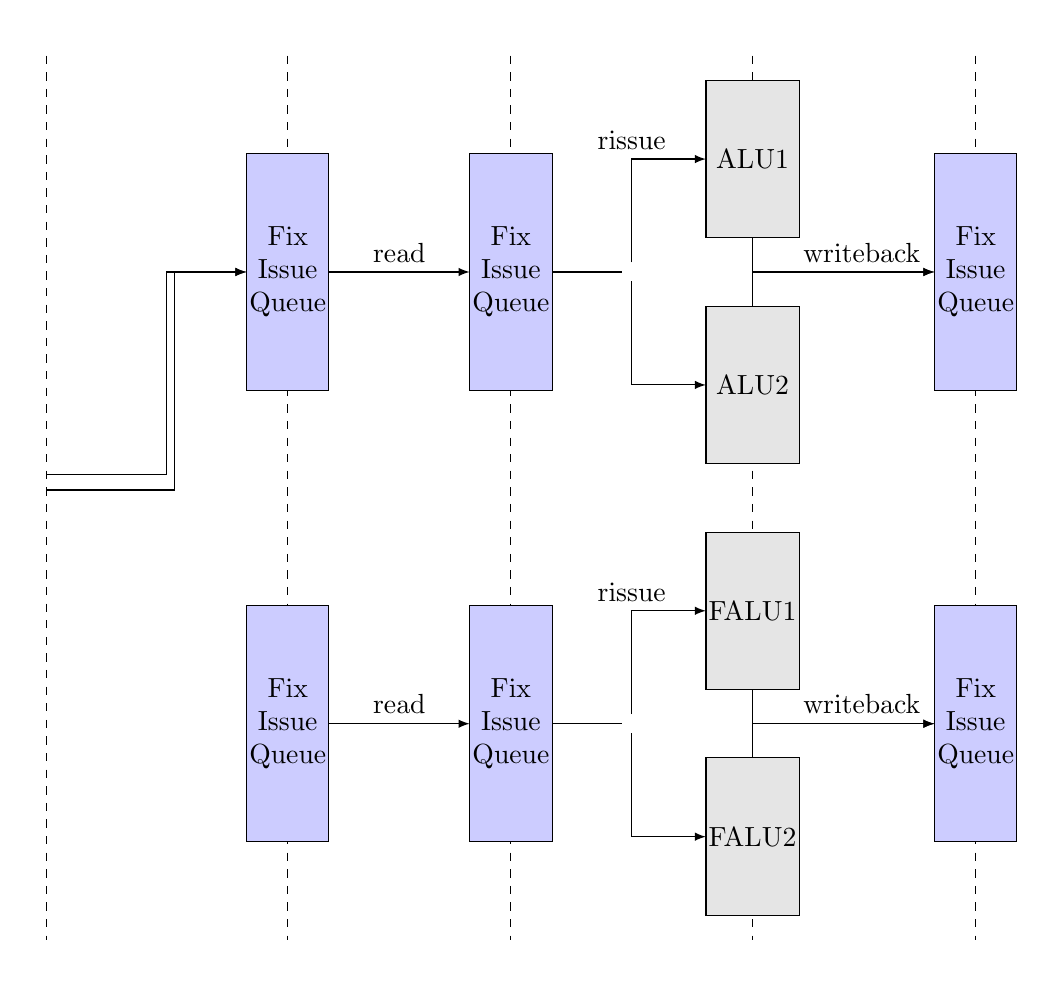
\begin{tikzpicture}

% 1. matrix layout
\node[matrix,very thin,column sep=1.3cm,row sep=1.2cm] (matrix) at (0,0) {
\eb{u1} &         & \eb{u2}     &  & \eb{u3}     &         & \eb{u4}     &  & \eb{u5} \\
        &         &             &  &             &         & \eb{mALU1}  &  & \\
        &         & \eb{mFixQ1} &  & \eb{mFixF1} & \eb{n1} &             &  & \eb{mFixF2} \\
        &         &             &  &             &         & \eb{mALU2}  &  & \\
\eb{m1} & \eb{m2} &             &  &             &         &             &  & \\
        &         &             &  &             &         & \eb{mFALU1} &  & \\
        &         & \eb{mFltQ1} &  & \eb{mFltF1} & \eb{n2} &             &  & \eb{mFltF2} \\
        &         &             &  &             &         & \eb{mFALU2} &  & \\
\eb{b1} &         & \eb{b2}     &  & \eb{b3}     &         & \eb{b4}     &  & \eb{b5} \\
};

% 2. vertical lines
\draw [dashed] 
  (u1) -- (b1) (u2) -- (b2) (u3) -- (b3) (u4) -- (b4) (u5) -- (b5);

% 3. align block boxes -- use \foreach later
\node[file] (FixQ1) at (mFixQ1) {Fix\\ Issue\\ Queue};
\node[file] (FltQ1) at (mFltQ1) {Fix\\ Issue\\ Queue};
\node[file] (FixF1) at (mFixF1) {Fix\\ Issue\\ Queue};
\node[file] (FltF1) at (mFltF1) {Fix\\ Issue\\ Queue};
\node[file] (FixF2) at (mFixF2) {Fix\\ Issue\\ Queue};
\node[file] (FltF2) at (mFltF2) {Fix\\ Issue\\ Queue};
\node[unit] (ALU1)  at (mALU1)  {ALU1};
\node[unit] (ALU2)  at (mALU2)  {ALU2};
\node[unit] (FALU1) at (mFALU1) {FALU1};
\node[unit] (FALU2) at (mFALU2) {FALU2};

% 4. arrows and label
\draw [-latex] (FixQ1) -- (FixF1) node[midway,above] {read};
\draw [-latex] (FltQ1) -- (FltF1) node[midway,above] {read};
\draw [-latex] (FixF1) -- (n1) |- (ALU1) node[midway,above] {rissue};
\draw [-latex] (FixF1) -- (n1) |- (ALU2);
\draw [-latex] (FltF1) -- (n2) |- (FALU1) node[midway,above] {rissue};
\draw [-latex] (FltF1) -- (n2) |- (FALU2);
\draw [-latex] (ALU1)  |- (FixF2) node[pos=0.8,above] {writeback};
\draw [-latex] (ALU2)  |- (FixF2);
\draw [-latex] (FALU1) |- (FltF2) node[pos=0.8,above] {writeback};
\draw [-latex] (FALU2) |- (FltF2);

\coordinate (m1) at ($(m1)$);
\coordinate (m2) at ($(m2)$);
\draw [-latex] ($(m1)+(0, .3)$) -- ($(m2)+( 0,.3)$) |- (FixQ1);
\draw [-latex] ($(m1)+(0, .1)$) -- ($(m2)+(.1,.1)$) |- (FixQ1);

\end{tikzpicture}
\end{document}

